\documentclass[11pt]{article}
\usepackage{euscript}
\usepackage{amsmath}
\usepackage{amsthm}
\usepackage{amssymb}
\usepackage{epsfig}
\usepackage{xspace}
\usepackage{amsmath,amssymb,amsthm}
\usepackage{graphicx}
\usepackage[margin=1in]{geometry}
\usepackage{fancyhdr}
\usepackage{color}
\usepackage{url}
\usepackage{bbm}
%%%%%%%%%%%%%%%%%%%%%%%%%%%%%%%%%
\setlength{\textheight}{9in}
\setlength{\topmargin}{-0.600in}
\setlength{\headheight}{0.2in}
\setlength{\headsep}{0.250in}
\setlength{\footskip}{0.5in}
\flushbottom
\setlength{\textwidth}{6.5in}
\setlength{\oddsidemargin}{0in}
\setlength{\evensidemargin}{0in}
\setlength{\columnsep}{2pc}
\setlength{\parindent}{1em}
\setlength{\parindent}{0pt}
\setlength{\parskip}{5pt plus 1pt}
\setlength{\headheight}{13.6pt}
%%%%%%%%%%%%%%%%%%%%%%%%%%%%%%%%%
\usepackage{epsfig}
\usepackage{xspace}
\usepackage{amsmath,amssymb,amsthm}
\usepackage{graphicx}
\usepackage[margin=1in]{geometry}
\usepackage{fancyhdr}
\usepackage{color}
\usepackage{url}
%%%%%%%  For drawing trees  %%%%%%%%%
\usepackage{tikz}
\usetikzlibrary{calc, shapes, backgrounds}
%%%%%%%%%%%%%%%%%%%%%%%%%%%%%%%%%
\setlength{\textheight}{9in}
\setlength{\topmargin}{-0.600in}
\setlength{\headheight}{0.2in}
\setlength{\headsep}{0.250in}
\setlength{\footskip}{0.5in}
\flushbottom
\setlength{\textwidth}{6.5in}
\setlength{\oddsidemargin}{0in}
\setlength{\evensidemargin}{0in}
\setlength{\columnsep}{2pc}
\setlength{\parindent}{1em}
\setlength{\parindent}{0pt}
\setlength{\parskip}{5pt plus 1pt}
\setlength{\headheight}{13.6pt}
%%%%%%%%%%%%%%%%%%%%%%%%%%%%%%%%%
\newcommand{\eps}{\varepsilon}
\renewcommand{\c}[1]{\ensuremath{\EuScript{#1}}}
\renewcommand{\b}[1]{\ensuremath{\mathbb{#1}}}
\renewcommand{\theenumi}{\alph{enumi}}
\newcommand{\s}[1]{\textsf{#1}}
\newcommand{\E}{\textbf{\textsf{E}}}
\renewcommand{\Pr}{\textbf{\textsf{Pr}}}
\newcommand\question[2]{\vspace{.25in}\hrule\textbf{#1: #2}\vspace{.5em}\hrule\vspace{.10in}}
\renewcommand\part[1]{\vspace{.10in}\textbf{(#1)}}
\newcommand\algorithm{\vspace{.10in}\textbf{Algorithm: }}
\newcommand\correctness{\vspace{.10in}\textbf{Correctness: }}
\newcommand\runtime{\vspace{.10in}\textbf{Running time: }}
\pagestyle{fancyplain}

\usepackage{listings}
\usepackage{color}

\definecolor{dkgreen}{rgb}{0,0.6,0}
\definecolor{gray}{rgb}{0.5,0.5,0.5}
\definecolor{mauve}{rgb}{0.58,0,0.82}

\lstset{frame=tb,
  language=Python,
  aboveskip=3mm,
  belowskip=3mm,
  showstringspaces=false,
  columns=flexible,
  basicstyle={\small\ttfamily},
  numbers=none,
  numberstyle=\tiny\color{gray},
  keywordstyle=\color{blue},
  commentstyle=\color{dkgreen},
  stringstyle=\color{mauve},
  breaklines=true,
  breakatwhitespace=true,
  tabsize=3
}

\graphicspath{ {.} }

\lhead{\textbf{\NAME\ (\UNI)}}
\chead{\textbf{HW\HWNUM}}
\rhead{COMS W4721, \today}


\newcommand\NAME{Daniel Kronovet}  
\newcommand\UNI{003349897}    
\newcommand\HWNUM{05}          

\begin{document}

%%%%%%%%%%%%%%%%%%%%%%%%%%%%%%%%%%%%%%%%%%%%%%%%%%%%
%%%%%%%%%%%%%%%%%%%%%%%%%%%%%%%%%%%%%%%%%%%%%%%%%%%%
%%%%%%%%%%%%%%%%%%%%%%%%%%%%%%%%%%%%%%%%%%%%%%%%%%%%

\section*{Problem 1 (K-Means)}

\subsection*{Part 1}

Plot the value of the objective function for K = 2,3,4,5 run over 20 iterations:
	
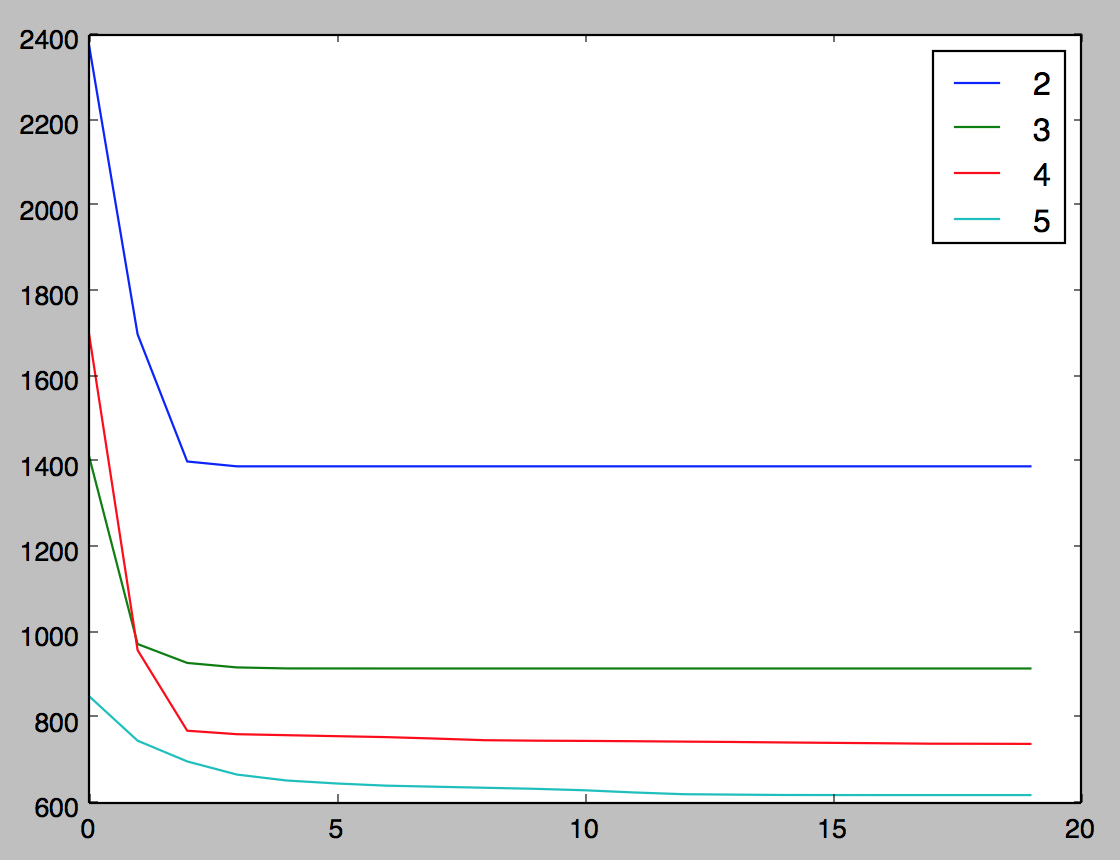
\includegraphics[scale=.5]{images/km_objective.png}

\subsection*{Part 2}

For k = 3, 5, plot the 500 data points and indicate the means:
		
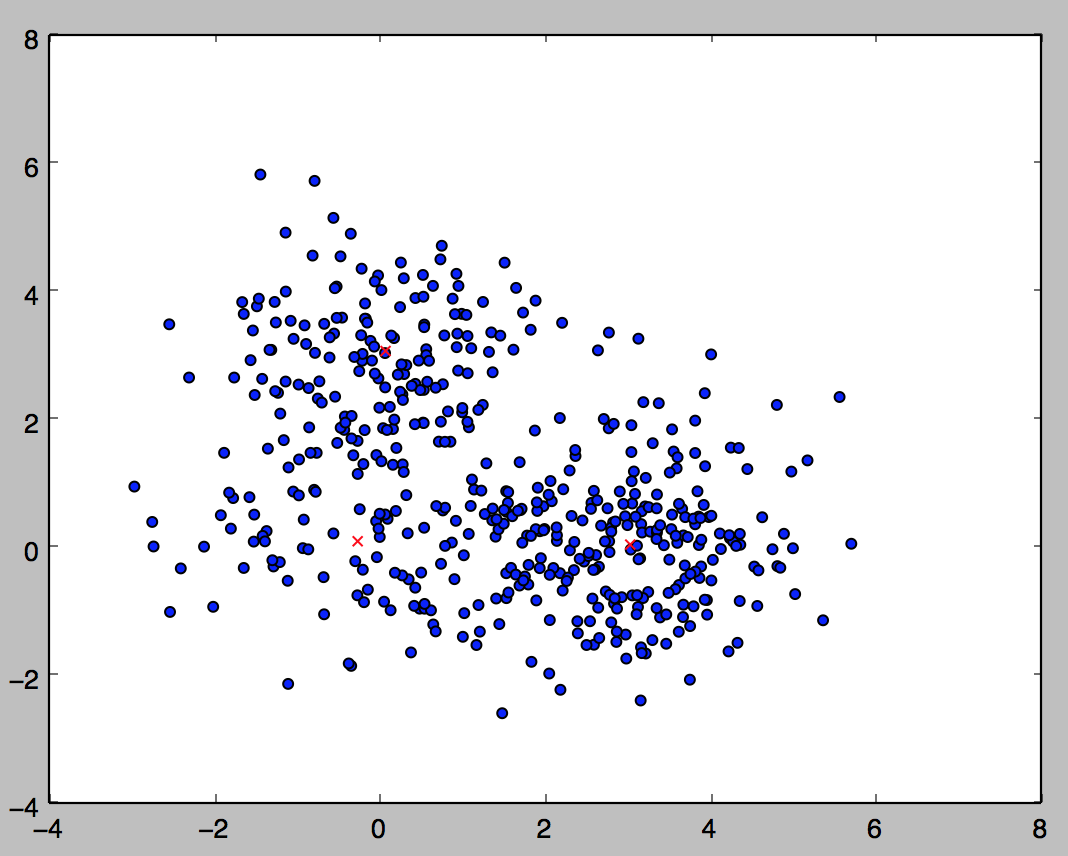
\includegraphics[scale=.5]{images/k3}

K=3

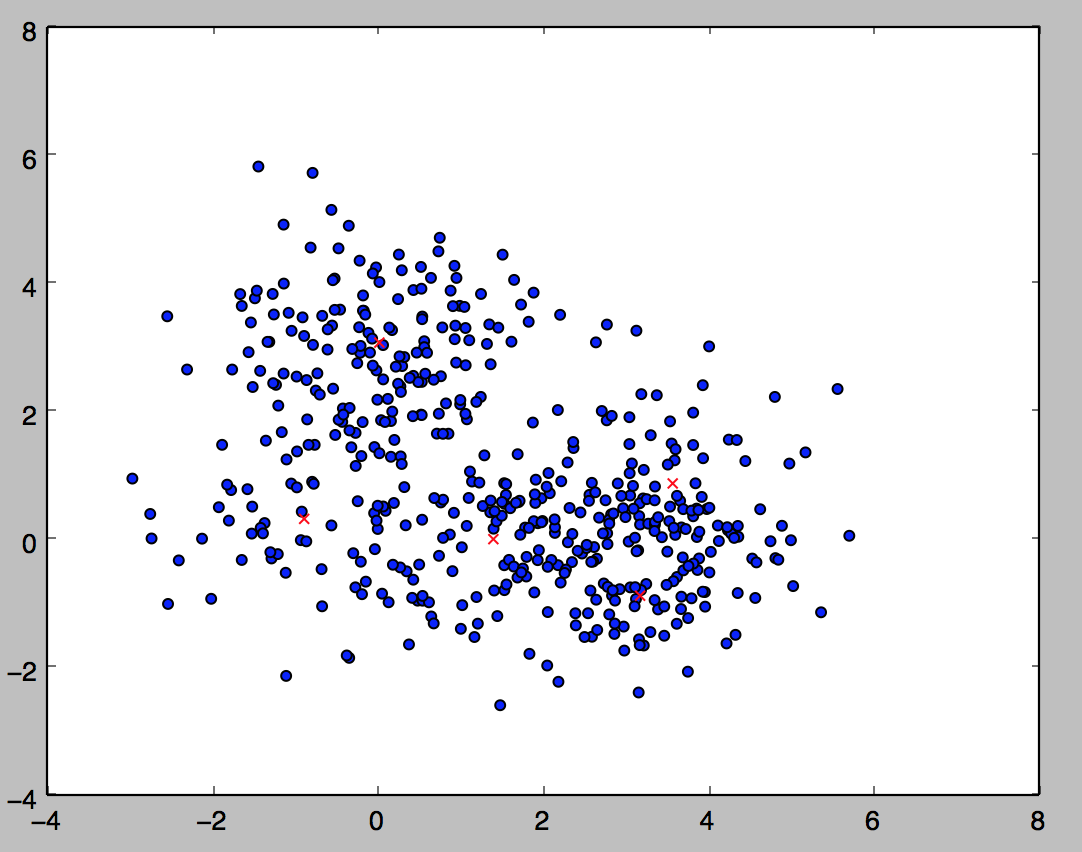
\includegraphics[scale=.5]{images/k5}

K=5

\section*{Problem 2 (Matrix Factorization)}

\subsection*{Part 1}

Plot the RMSE of your predictions on this test set as a function of training iteration. On a separate plot show the log joint likelihood as a function of iteration.

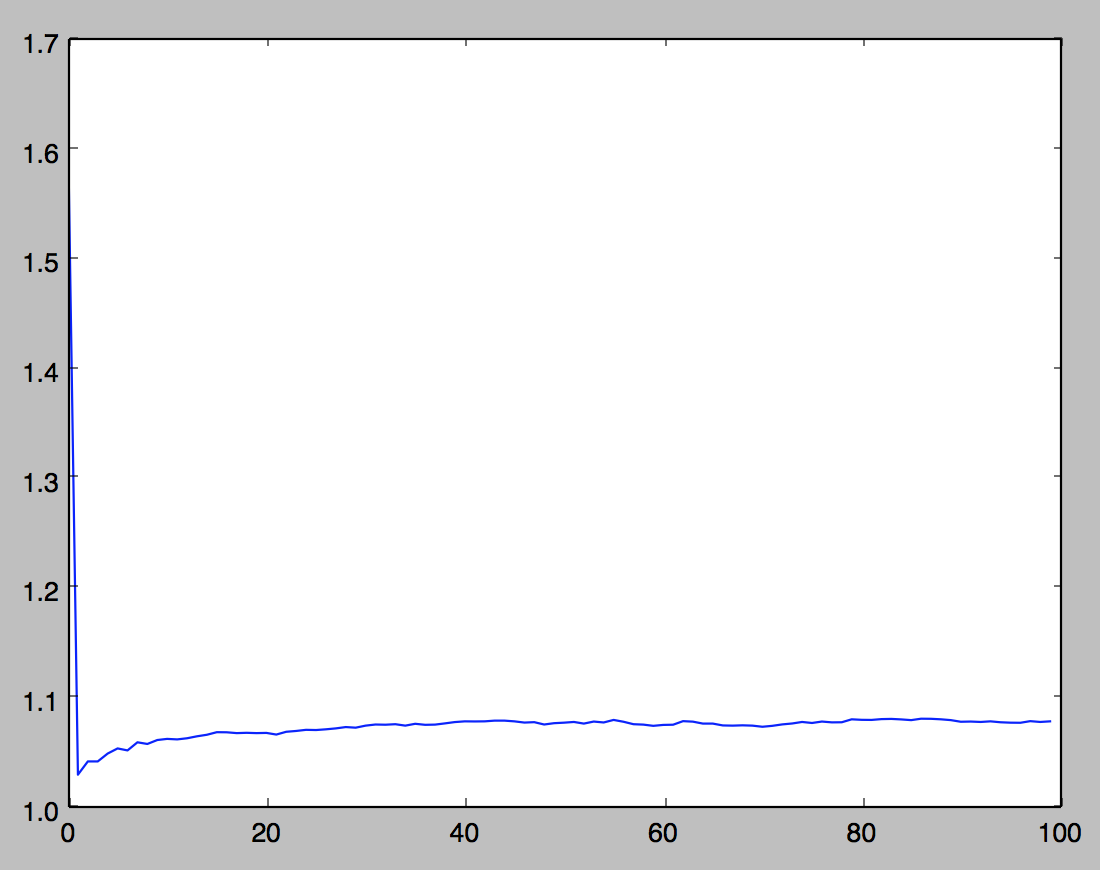
\includegraphics[scale=.5]{images/rmse}

Root Mean Square Error

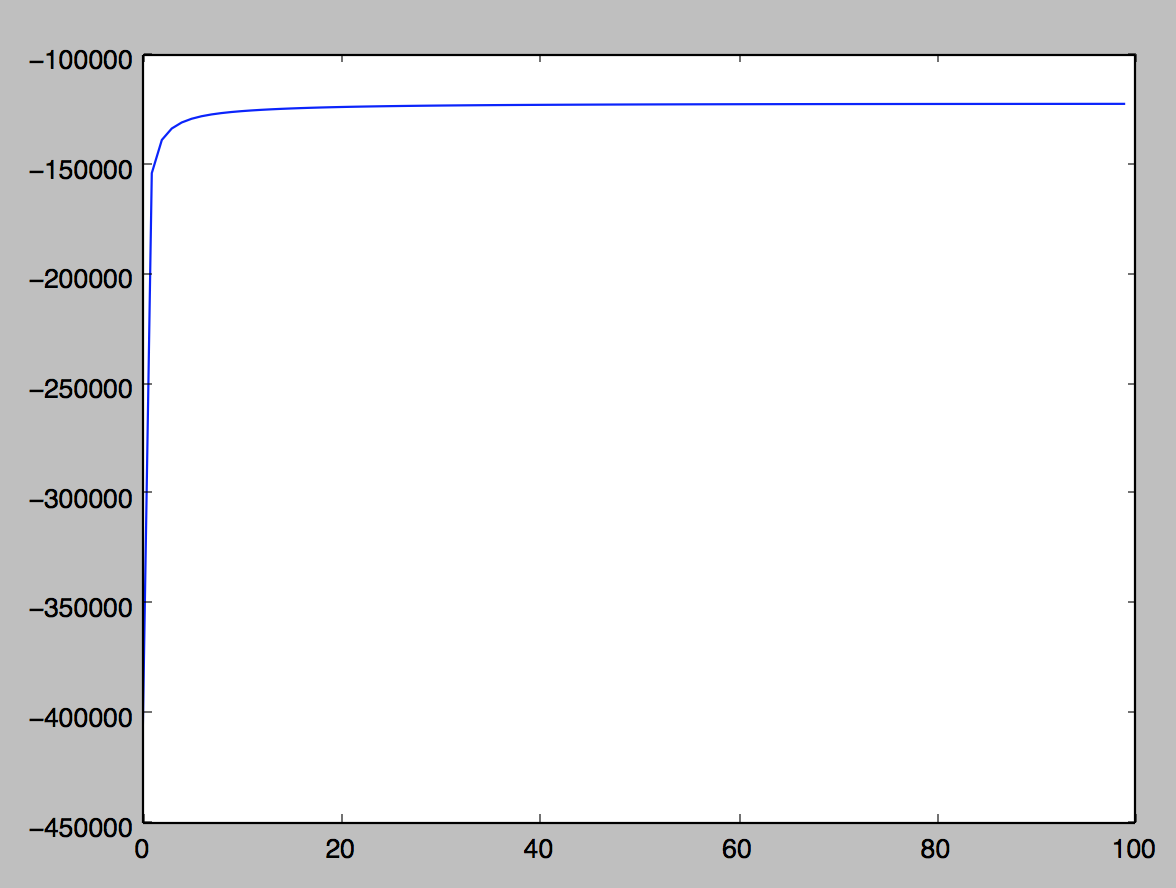
\includegraphics[scale=.5]{images/ljl}

Log Joint Likelihood

\subsection*{Part 2}

Pick three movies and for each movie find the 5 closest movies according to Euclidean distance using their respective locations $v_i$. List the query movie, the five nearest movies and their distances. A mapping from index to movie is given with the data.

\textbf{American President, The (1995)}:

- 'Boogie Nights (1997)': 12.289614399025282,

 - 'Everyone Says I Love You (1996)': 11.256697317789136,

 - 'Jackie Brown (1997)': 11.845881441814806,

 - 'Leaving Las Vegas (1995)': 11.502639879587134,

 - 'Lost Highway (1997)': 11.508749002317485
 
 ---
 
\textbf{Once Upon a Time in America (1984)}:

- 'Crash (1996)': 9.7582811139410222,

- 'Everyone Says I Love You (1996)': 10.965926355087346,

- 'Evita (1996)': 13.883277684441039,

- 'Mother (1996)': 9.8714055212553244,

- 'Saint, The (1997)': 10.060582911571393
 
 ---
 
\textbf{Ben-Hur (1959)}:

- 'English Patient, The (1996)': 13.334206228955669,

- 'Everyone Says I Love You (1996)': 13.030630831731056,

- 'Evita (1996)': 13.373182102561227,

- 'Lost Highway (1997)': 12.99448128577829,

- 'Mother (1996)': 15.102456207015678

\subsection*{Part 3}

Perform K-means on the $u_1, . . . , u_{N1}$ learned by your algorithm. Set $K$ = 30. The centroids can be interpreted as personality types (as far as movies are concerned). Pick 5 centroids. For each centroid, characterize the cluster by showing the 10 movies with the largest (most positive) dot product to that centroid.	

\textbf{Centroid 3}:

[('Godfather, The (1972)', 4.7184533749610802),

     ('L.A. Confidential (1997)', 4.5925149458403443),
     
     ('Jackie Brown (1997)', 4.5322949319352333),
 
     ('Godfather: Part II, The (1974)', 4.524063347210312),
 
     ("One Flew Over the Cuckoo's Nest (1975)", 4.4742673268931075),
 
     ('North by Northwest (1959)', 4.4215418122679981),
 
     ('Silence of the Lambs, The (1991)', 4.3993152612511812),
 
     ('Psycho (1960)', 4.3845790178796502),
 
     ('High Noon (1952)', 4.3529535156264556),
 
     ('Raging Bull (1980)', 4.3204443198774909)],
     
     ---
     
\textbf{Centroid 4}:
 
 [('Silence of the Lambs, The (1991)', 4.557299992895854),
 
     ('Henry V (1989)', 4.4646471922267148),
 
     ('Usual Suspects, The (1995)', 4.462597884519143),
 
     ('Die Hard (1988)', 4.4612785815183456),
 
     ('Blues Brothers, The (1980)', 4.4327461814166851),
 
     ('Shawshank Redemption, The (1994)', 4.4261339426801074),
 
     ('Nikita (La Femme Nikita) (1990)', 4.3959800821438479),
 
     ('Fugitive, The (1993)', 4.3925052555952107),
 
     ('Terminator 2: Judgment Day (1991)', 4.3770856236760061),
 
     ('Day the Earth Stood Still, The (1951)', 4.3667358807077434)],
     
     ---
     
\textbf{Centroid 19}:
 
 [('Absolute Power (1997)', 5.3246857746580174),
 
      ("Jackie Chan's First Strike (1996)", 5.2618901041844115),
 
      ('Wedding Singer, The (1998)', 5.1677201794345562),
 
      ('Aristocats, The (1970)', 4.9388278307790934),
 
      ('Immortal Beloved (1994)', 4.8405296710573822),
 
      ('Babe (1995)', 4.8244986246259387),
 
      ('Sound of Music, The (1965)', 4.7967544449427972),
 
      ('Replacement Killers, The (1998)', 4.767350531353407),
 
      ('Kingpin (1996)', 4.7179323871595393),
 
      ('Conspiracy Theory (1997)', 4.7139296230923238)],
      
      ---
      
\textbf{Centroid 20}:
 
 [('Dr. Strangelove or: How I Learned to Stop Worrying and Love the Bomb (1963)', 4.6828018823687412),
 
      ('Close Shave, A (1995)', 4.6549510725637795),
 
      ('Citizen Kane (1941)', 4.628284564385325),
 
      ('Lawrence of Arabia (1962)', 4.5000488815891675),
 
      ('Rear Window (1954)', 4.4890186194668917),
 
      ('Wrong Trousers, The (1993)', 4.4880402007879052),
 
      ('Godfather, The (1972)', 4.484296146401471),
 
      ('Kolya (1996)', 4.4650279836087741),
 
      ('Lone Star (1996)', 4.4584969668617465),
 
      ('North by Northwest (1959)', 4.4536776645909484)],
      
      ---
 
\textbf{Centroid 21}:
 
 [('Fast, Cheap, and Out of Control (1997)', 5.4954521220655863),
 
      ('Alien (1979)', 5.2681630706563194),
 
      ('Big Sleep, The (1946)', 5.1120579475632724),
 
      ('12 Angry Men (1957)', 5.0446240885383631),
 
      ('Psycho (1960)', 5.0232558189519914),
 
      ('Crash (1996)', 5.0206367903721913),
 
      ('North by Northwest (1959)', 5.0202825687314139),
 
      ('Bride of Frankenstein (1935)', 4.9890033207285729),
 
      ('Citizen Kane (1941)', 4.9778390450581531),
 
      ('Terminator 2: Judgment Day (1991)', 4.9686310854118272)]

\end{document}
